% Architecture figure. Compile separately: pdflatex architecture.tex
%
% A uniform grid of framed items. Each frame carries the colour of its role, holds a picture of what
% it computes on the left, and its name over one short line on the right.
%   columns [0.15,5.55] [6.45,11.85] [12.75,18.15]     rows y = 0 / -3.2 / -6.4 / -9.3
%   row 1 perception, row 2 the three heads, row 3 the geometric route and the fusion
%   (each under the head that feeds it), row 4 the given mesh, the colour key, the output.
\documentclass[tikz,border=2pt]{standalone}
\usepackage{amsmath,amssymb,xcolor,graphicx,helvet}
\renewcommand{\familydefault}{\sfdefault}
% Notation (docs/07): keep consistent across text, figures and tables.
\newcommand{\PaperTitle}{Factored Interaction Fields: Learning Joint-Anchored Hand-Object Proximity Through Its Geometric Arguments}
\newcommand{\method}{FIF}
\newcommand{\field}{\mathbf{v}}
\newcommand{\joint}{\mathbf{p}}
\newcommand{\vtx}{\mathbf{q}}
\newcommand{\objpose}{\theta_o}
\newcommand{\Rot}{\mathbf{R}}
\newcommand{\trans}{\mathbf{t}}
\newcommand{\mesh}{\mathcal{Q}}
\newcommand{\ade}{\mathrm{ADE}}
\newcommand{\mm}{\,\mathrm{mm}}
\newcommand{\ie}{i.e.}
\newcommand{\eg}{e.g.}

\usetikzlibrary{arrows.meta,calc,backgrounds}

\definecolor{cGiven}{HTML}{2F6DB0}
\definecolor{cTrain}{HTML}{6E4E9B}
\definecolor{cGeom}{HTML}{1F8274}
\definecolor{cFuse}{HTML}{C1762A}
\definecolor{cInk}{HTML}{23282F}
\definecolor{cBody}{HTML}{4E545B}
\definecolor{cRule}{HTML}{BFC5CB}
\definecolor{cLoss}{HTML}{A8322D}
\newcommand{\m}[1]{\mbox{$#1$}}

\begin{document}
\hyphenpenalty=10000\exhyphenpenalty=10000\relax
\begin{tikzpicture}[x=1cm,y=1cm,
  frame/.style={draw, rounded corners=3pt, line width=0.8pt, fill=white, inner sep=0},
  arr/.style={-{Latex[length=2.1mm,width=1.7mm]}, line width=0.75pt, draw=cInk!75},
  wire/.style={line width=0.75pt, draw=cInk!75},
  tag/.style={font=\scriptsize, text=cBody, inner sep=1.5pt},
  ico/.style={x=1mm, y=1mm, sharp corners, line cap=round, line join=round, line width=0.6pt},
]
% frame of one item:  #1 centre, #2 role colour, #3 height in mm
\def\itemframe#1#2#3{\node[frame, draw=#2, minimum width=54mm, minimum height=#3mm] at #1 {};}
% picture well inside an item: #1 centre, #2 role colour, #3 height in mm
\def\well#1#2#3{\node[draw=#2!35, fill=#2!6, rounded corners=2pt, line width=0.5pt, inner sep=0,
  minimum width=18mm, minimum height=#3mm] at #1 {};}
% name and one line, set beside the picture
\def\lab#1#2#3#4{\node[anchor=west, text width=28mm, align=left, inner sep=0] at #1
  {\textbf{\footnotesize\color{#2}#3}\\[0.6mm]{\scriptsize\color{cBody}#4}};}

% ================================================== row 1: perception (y = 0)
\itemframe{(2.85,0)}{cGiven}{21}   \well{(1.30,0)}{cGiven}{17}
\node[inner sep=0, draw=white, line width=1.1pt] at (1.39,-0.09) {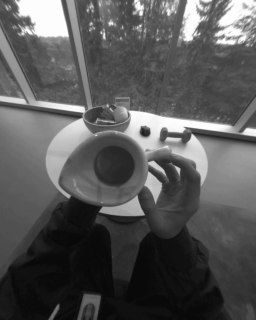
\includegraphics[width=10.2mm]{thumb_in1.png}};
\node[inner sep=0, draw=white, line width=1.1pt] at (1.21,0.09) {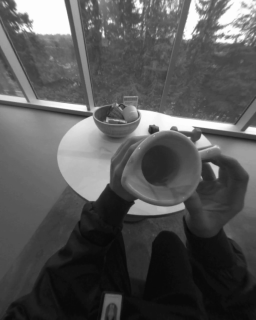
\includegraphics[width=10.2mm]{thumb_in0.png}};
\lab{(2.40,0)}{cGiven}{stereo input}{two synchronised headset views, $1024{\times}1280$, calibrated}

\itemframe{(9.15,0)}{cGiven}{21}   \well{(7.60,0)}{cGiven}{17}
\node[inner sep=0] at (7.28,0) {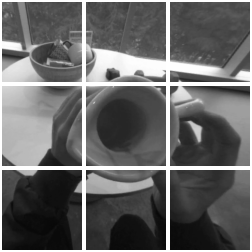
\includegraphics[width=11.6mm]{thumb_patches.png}};
\foreach \y in {0.33,0.11,-0.11,-0.33}{\draw[draw=cGiven, fill=white, rounded corners=0.8pt, line width=0.45pt] (8.02,\y-0.08) rectangle ++(0.36,0.16);}
\draw[arr, line width=0.45pt, -{Latex[length=1.2mm,width=1.0mm]}] (7.88,0) -- (7.97,0);
\lab{(8.70,0)}{cGiven}{frozen tokens}{DINOv3 ViT-B/16 patches of both views, each tagged with its Pl\"ucker ray}

\itemframe{(15.45,0)}{cTrain}{21}  \well{(13.90,0)}{cTrain}{17}
\foreach \a/\b in {0/0,0/1,1/1,1/2,2/2,2/3,3/3,3/4,4/4,4/5,0/2,2/4,3/1}{%
  \draw[cTrain!40, line width=0.35pt] (13.12+\a*0.39,0.40) -- (13.12+\b*0.312,-0.40);}
\foreach \i in {0,1,2,3,4}{\fill[cTrain] (13.12+\i*0.39,0.40) circle (0.07);}
\foreach \i in {0,1,2,3,4,5}{\draw[cTrain, fill=white, line width=0.45pt] (13.12+\i*0.312-0.07,-0.47) rectangle ++(0.14,0.14);}
\lab{(15.00,0)}{cTrain}{transformer decoder}{$L{=}6$ layers, 42 joint and 16 object queries}

\draw[arr] (5.55,0) -- (6.45,0);
\draw[arr] (11.85,0) -- (12.75,0);

% ================================================== row 2: the three heads (y = -3.2)
\itemframe{(2.85,-3.2)}{cTrain}{21}  \well{(1.30,-3.2)}{cTrain}{17}
\begin{scope}[ico, shift={(1.30cm,-3.2cm)}]
  \draw[cTrain!65, line width=0.4pt] (90:5.6) -- (162:5.6) -- (234:5.6) -- (306:5.6) -- (18:5.6) -- cycle;
  \foreach \a in {90,162,234,306,18}{\draw[cTrain!45, line width=0.35pt] (0,0) -- (\a:5.6);}
  \foreach \a in {90,162,234,306,18}{\fill[cTrain] (\a:5.6) circle (1.05);}
  \fill[cTrain!60] (0,0) circle (0.85);
\end{scope}
\lab{(2.40,-3.2)}{cTrain}{object control-point head}{control points $\hat{\mathbf{c}}_n$ with confidences $w_n$}

\itemframe{(9.15,-3.2)}{cTrain}{21}  \well{(7.60,-3.2)}{cTrain}{17}
\begin{scope}[ico, shift={(7.60cm,-3.2cm)}]
  \foreach \c in {{(-4.0,-2.9),(-5.5,-0.8),(-6.2,1.0)},{(-2.1,-1.1),(-2.4,1.6),(-2.6,4.1)},%
                  {(0,-0.9),(0,2.0),(0,5.0)},{(2.1,-1.1),(2.4,1.6),(2.6,4.1)},{(3.9,-2.1),(4.6,0.3),(4.9,2.6)}}{%
    \draw[cTrain, line width=0.5pt] (0,-5.4) \foreach \p in \c {-- \p};
    \foreach \p in \c {\fill[cTrain] \p circle (0.64);}}
  \fill[cTrain] (0,-5.4) circle (0.9);
\end{scope}
\lab{(8.70,-3.2)}{cTrain}{joint head}{camera-frame hand joints $\hat{\joint}_{h,j}$, in millimetres}

\itemframe{(15.45,-3.2)}{cTrain}{21} \well{(13.90,-3.2)}{cTrain}{17}
\begin{scope}[ico, shift={(13.90cm,-3.2cm)}]
  \draw[cTrain!55, dash pattern=on 0.7mm off 0.45mm, line width=0.45pt] (2.8,2.8) circle (2.7);
  \draw[cTrain, -{Latex[length=2.0mm,width=1.6mm]}, line width=0.9pt] (-4.8,-4.8) -- (2.7,2.7);
  \fill[cTrain] (-4.8,-4.8) circle (1.0);
\end{scope}
\lab{(15.00,-3.2)}{cTrain}{direct head}{the field \m{\field^{\rm dir}} and its \mbox{log-scale} \m{s^{\rm dir}}}

\draw[wire, rounded corners=5pt] (15.45,-1.05) -- (15.45,-1.62) -- (2.85,-1.62);
\foreach \x in {2.85,9.15,15.45}{\draw[arr] (\x,-1.62) -- (\x,-2.15);}
\node[tag, anchor=south] at (12.1,-1.57) {refined queries};

% ================================================== row 3: geometry and fusion (y = -6.4)
\itemframe{(2.85,-6.4)}{cGeom}{21}  \well{(1.30,-6.4)}{cGeom}{17}
\begin{scope}[ico, shift={(1.30cm,-6.4cm)}]
  \draw[cGeom!50, densely dashed, line width=0.45pt] (-5.8,-4.9) -- (-1.2,-5.9) -- (-3.0,-1.4) -- cycle;
  \foreach \p in {(-5.8,-4.9),(-1.2,-5.9),(-3.0,-1.4)}{\draw[cGeom!70, fill=white, line width=0.45pt] \p circle (0.85);}
  \draw[cGeom] (1.4,0.7) -- (6.0,1.8) -- (2.8,5.6) -- cycle;
  \foreach \p in {(1.4,0.7),(6.0,1.8),(2.8,5.6)}{\fill[cGeom] \p circle (0.9);}
  \draw[cGeom, -{Latex[length=1.8mm,width=1.5mm]}, line width=0.65pt] (-2.8,0.7) to[bend left=32] (0.6,3.9);
\end{scope}
\lab{(2.40,-6.4)}{cGeom}{weighted Procrustes}{object pose \m{(\hat{\Rot}_o,\hat{\trans}_o)} in closed form, differentiable}

\itemframe{(9.15,-6.4)}{cGeom}{21}  \well{(7.60,-6.4)}{cGeom}{17}
\begin{scope}[ico, shift={(7.60cm,-6.4cm)}]
  \foreach \a/\b in {{(-6.2,1)}/{(-3.1,4.2)},{(-3.1,4.2)}/{(0,1.5)},{(0,1.5)}/{(3.1,4.8)},{(3.1,4.8)}/{(6.2,1)},%
                     {(6.2,1)}/{(2.1,-1.3)},{(2.1,-1.3)}/{(-2.1,-1.8)},{(-2.1,-1.8)}/{(-6.2,1)},%
                     {(-3.1,4.2)}/{(-2.1,-1.8)},{(0,1.5)}/{(-2.1,-1.8)},{(0,1.5)}/{(2.1,-1.3)},{(3.1,4.8)}/{(2.1,-1.3)}}{%
    \draw[cGeom!55, line width=0.4pt] \a -- \b;}
  \foreach \p in {(-6.2,1),(-3.1,4.2),(3.1,4.8),(6.2,1),(2.1,-1.3),(-2.1,-1.8)}{\fill[cGeom!80] \p circle (0.62);}
  \draw[cGeom!45, dash pattern=on 0.7mm off 0.45mm, line width=0.45pt] (0,1.5) circle (2.7);
  \fill[cGeom] (0,1.5) circle (1.05);
  \draw[cGeom, -{Latex[length=1.9mm,width=1.5mm]}, line width=0.85pt] (-1.0,-6.6) -- (-0.15,-0.2);
  \fill[cTrain] (-1.0,-6.6) circle (1.0);
\end{scope}
\lab{(8.70,-6.4)}{cGeom}{soft nearest vertex}{the geometric field \m{\field^{\rm geo}}, evaluated on the posed mesh}

\itemframe{(15.45,-6.4)}{cFuse}{21} \well{(13.90,-6.4)}{cFuse}{17}
\begin{scope}[ico, shift={(13.90cm,-6.4cm)}]
  \draw[cRule, line width=0.4pt] (-7.0,-5.2) -- (7.0,-5.2);
  \draw[cGeom, line width=0.75pt] plot[domain=-7.0:7.0,samples=48,smooth] (\x,{-5.2+4.4*exp(-pow(\x-2.4,2)/14.0)});
  \draw[cTrain, line width=0.75pt] plot[domain=-7.0:7.0,samples=48,smooth] (\x,{-5.2+10.2*exp(-pow(\x+2.1,2)/2.6)});
  \draw[cFuse, line width=0.9pt] (-1.4,-5.7) -- (-1.4,5.8);
  \fill[cFuse] (-1.4,5.8) circle (0.75);
\end{scope}
\lab{(15.00,-6.4)}{cFuse}{precision-weighted fusion}{per-joint weights \m{\lambda^{k}=e^{-2s^{k}}} from the predicted scales}

\foreach \x in {2.85,9.15,15.45}{\draw[arr] (\x,-4.25) -- (\x,-5.35);}
\draw[arr] (5.55,-6.4) -- (6.45,-6.4);
\draw[arr] (11.85,-6.4) -- (12.75,-6.4);

% ================================================== row 4: given mesh, key, output (y = -9.3)
\itemframe{(2.85,-9.3)}{cGiven}{19} \well{(1.30,-9.3)}{cGiven}{15}
\node[inner sep=0] at (1.30,-9.3) {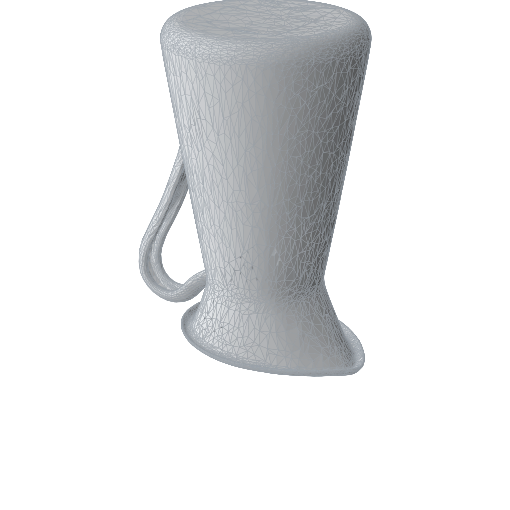
\includegraphics[width=13mm]{thumb_meshgrey.png}};
\lab{(2.40,-9.3)}{cGiven}{canonical mesh}{given with the object alias: 16 control points, 1{,}024 vertices}
\draw[arr] (2.85,-8.35) -- (2.85,-7.55);

\node[frame, draw=cRule, minimum width=54mm, minimum height=19mm] at (9.15,-9.3) {};
\foreach \y/\c/\t in {-8.72/cGiven/{frozen or given}, -9.12/cTrain/{trained},
                      -9.52/cGeom/{differentiable geometry, no parameters}, -9.92/cFuse/{fusion}}{%
  \draw[draw=\c, fill=\c!15, rounded corners=1.2pt, line width=0.7pt] (6.95,\y-0.10) rectangle ++(0.48,0.20);
  \node[tag, anchor=west] at (7.58,\y) {\t};}

\itemframe{(15.45,-9.3)}{cFuse}{19} \well{(13.90,-9.3)}{cFuse}{15}
\node[inner sep=0] at (13.90,-9.3) {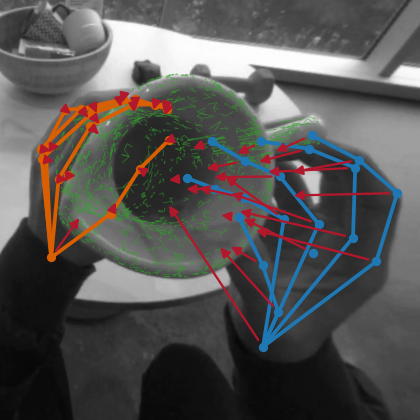
\includegraphics[width=13.6mm]{thumb_out.png}};
\lab{(15.00,-9.3)}{cFuse}{predicted field}{rotated into the world frame: \m{2{\times}21{\times}3} values in mm}
\draw[arr] (15.45,-7.45) -- (15.45,-8.25);

% ================================================== training note
\node[anchor=north, font=\scriptsize, text=cLoss] at (9.15,-10.45)
  {\textbf{training:} the endpoint error of the fused field, a Gaussian negative log-likelihood per head, and auxiliary losses on the three heads};
\end{tikzpicture}
\end{document}
